\documentclass[a4paper,14pt]{article}
\usepackage{extsizes}
\usepackage{amsmath}
\usepackage{amssymb}
\everymath{\displaystyle}
\usepackage{geometry}
\usepackage{fancyhdr}
\usepackage{multicol}
\usepackage{graphicx}
\usepackage[brazil]{babel}
\usepackage[shortlabels]{enumitem}
\usepackage{cancel}
\columnsep=2cm
\hoffset=0cm
\textwidth=8cm
\setlength{\columnseprule}{.1pt}
\setlength{\columnsep}{2cm}
\renewcommand{\headrulewidth}{0pt}
\geometry{top=1in, bottom=1in, left=0.7in, right=0.5in}

\pagestyle{fancy}
\fancyhf{}
\fancyfoot[C]{\thepage}

\begin{document}
	
	\noindent\textbf{7FMA153~-~Matemática} 
	
	\begin{center}Gráficos na forma de segmento de reta (Versão estudante)
	\end{center}
	
	
	\noindent\textbf{Nome:} \underline{\hspace{10cm}}
    \noindent\textbf{Data:} \underline{\hspace{4cm}}
	
	%\section*{Questões de Matemática}
	
	\begin{multicols}{2}
	    Observe este gráfico e resolva as questões de 1 a 5.
	    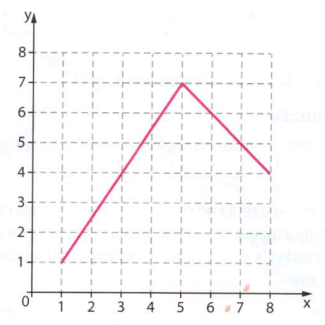
\includegraphics[width=0.45\textwidth]{/home/hogdelta/Documentos/latex/7FMA153_imagens/pg70.png}
	    \begin{enumerate}
	    	\item Determine $y$ quando $x = 3$ \\\\\\\\\\\\
	    	\item Ache $x$ quando $y = 5$ (no segundo segmento). \\\\\\\\\\
	    	\item Ache $x$ quando $y=1$ (no segundo segmento, podendo prolongá-lo para valores de $x$ maiores que 8). \\\\\\\\\\
	    	\item Calcule $y$ para $x = 3,5$ \\\\\\\\\\
	    	\item Descubra $y$ para $x = 6,2$. \\\\\\\\\\\\\\\\\\
	    	Texto p/ as questões de 6 a 9. \\\\
	    	Um pesquisador analisava duas culturas diferentes com o objetivo de verificar como ocorria a evolução, ao longo do tempo, do crescimento do número de bactérias presentes em cada uma das culturas, sob certas condições. Essa evolução foi representada no gráfico a seguir: 
	    	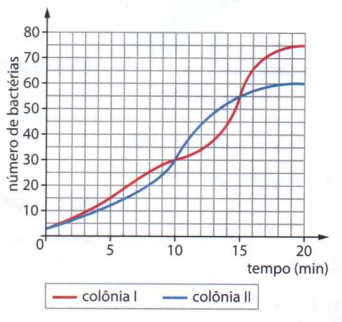
\includegraphics[width=0.45\textwidth]{/home/hogdelta/Documentos/latex/7FMA153_imagens/pg84.png}
	    	\item Qual é o número de bactérias presentes nas culturas observadas em 8 minutos?
	    	\item Em que intervalo de tempo o número de bactérias na colônia I foi menor do que o número de bactérias na colônia II?
	    	\item Determine o aumento percentual no número de bactérias na colônia I entre 15 minutos e 20 minutos.
	    	\item Determine o aumento percentual no número de bactérias da colônia II entre 10 minutos e 15 minutos.
	    	$~$ \\ $~$ \\ $~$ \\ $~$ \\ $~$ \\ $~$ \\ $~$ \\ $~$ \\ $~$ \\ $~$ \\ $~$ \\ $~$ \\ $~$ \\ $~$ \\ $~$ \\ $~$ \\ $~$ \\ $~$ \\ $~$ \\ $~$ \\ $~$ \\ $~$ \\ $~$ \\ $~$ \\ $~$ \\ $~$ \\ $~$ \\ $~$ \\ $~$ \\ $~$ \\ $~$ \\ $~$ \\ $~$ \\ $~$ \\ $~$ \\ $~$ \\ $~$ \\ $~$ \\ $~$ \\ $~$ \\ $~$ \\ $~$ \\ $~$ \\ $~$ \\ $~$ \\ $~$ \\ $~$ \\ $~$ \\ $~$ \\ $~$ \\ $~$ \\ $~$ \\ 
	    	
        \end{enumerate} 
    \end{multicols}
\end{document}